%%%%%%%%%%%%%%%%%%%%%%%%%%%%%% -*- Mode: Latex -*- %%%%%%%%%%%%%%%%%%%%%%%%%%%%
%% diss-intro.tex -- 
%% Author          : Carleton Moore
%% Created On      : Mon Oct  5 10:58:59 1998
%% Last Modified By: Carleton Moore
%% Last Modified On: Wed Oct 27 10:30:51 1999
%% RCS: $Id: diss-intro.tex,v 1.4 1999/10/27 20:30:54 cmoore Exp $
%%%%%%%%%%%%%%%%%%%%%%%%%%%%%%%%%%%%%%%%%%%%%%%%%%%%%%%%%%%%%%%%%%%%%%%%%%%%%%%
%%   Copyright (C) 1998 Carleton Moore
%%%%%%%%%%%%%%%%%%%%%%%%%%%%%%%%%%%%%%%%%%%%%%%%%%%%%%%%%%%%%%%%%%%%%%%%%%%%%%%
%% 

\chapter{Introduction}
\label{sec:intro}
\begin{quote}
{\em At the start, when we know much about the problem and nothing about the
solution, the solution is very abstract.} -- Robert H. Dunn
\end{quote}

Every software developer wishes they got home from work sooner and spent less
of their weekend at work. Software developers work very hard and very long, yet
software is often delivered late, over budget, and full of defects.  Over forty
years of software development experience has not helped us solve this problem.
How can software developers gain more control over their software development
and produce high quality software efficiently?  Project LEAP and the Leap
toolkit in particular attempts to give developers the control and skills they
need.  Before I discuss Leap I will give a short background of the software
development problem.

\section{Why is Quality Software Development Important?}



Software is controlling more safety critical tasks and important
functions\cite{Armour93}. Yet software errors occur sometimes with horrible
costs. Between 1985 and 1987 the Therac-25 radiation therapy machine killed two
people and seriously injured four others by delivering massive radiation
overdoses.  Investigations found that many issues were to blame including
faulty software\cite{Leveson93}.

In March 1995, the Denver International Airport opened over 16 months late and
over 100 million dollars over budget. One of the primary reasons for the delay
and overrun was the presence of major bugs in the baggage handling control
software\cite{Glass98}.

Another problem with current software development is productivity. The
insatiable demand for more software has out-paced our ability to produce
software.  Software productivity has not kept pace with hardware
cost/performance ratios. The most optimistic rate at which programmer
productivity is increasing is 5\% per year, while there is greater than a ten
fold increase in the demand for software each decade.\cite{Dunn90} The
government of the United States of America faces this problem. In 1996
Computerworld reported that delays in overhauling the federal tax computer
systems cost the U.S.  Treasury as much as \$50 billion per year.\cite{Glass98}
The problem of overhauling of the tax computers is not purely a software issue
but the software system is a large part of the problem.

\section{Traditional Solutions}

Software developers and managers have addressed software quality and
development issues since the beginning of the computer age. Developer and
managers have continuously augmented the development methods they use. We can
divide these methods into four eras: hope-based, product-based,
organization-based, and individual-based.  Figure \ref{fig:eras} shows a time
line of software development improvement and the different eras.

\begin{center}
  \begin{figure}[htb]
    \setlength{\unitlength}{2.5cm}
    \begin{picture}(6,3)
      \setlength{\fboxsep}{0.25cm}
      \thicklines
      \put(0.25,1.5){\vector(1,0){5.5}}
      \thinlines
      \put(5.6,1.6){Time}
      \put(1,1.5){\circle*{0.15}}
      \put(1.3,1.6){1960s}
      \put(2,1.5){\circle*{0.15}}
      \put(2.3,1.3){1970s}
      \put(3,1.5){\circle*{0.15}}
      \put(3.3,1.6){1980s}
      \put(4,1.5){\circle*{0.15}}
      \put(4.3,1.3){1990s}
      \put(5,1.5){\circle*{0.15}}
      \put(0.9,0.25){\framebox(1.25,0.5){\parbox[b]{2.5cm}{Hope-based (Try
            harder)}}}
      \put(1.2,0.8){\begin{picture}(0.75, 0.75)
          \put(0.25,0){\line(0,1){0.3}}
          \put(0.5,0){\line(0,1){0.3}}
          \put(0.05,0.3){\line(1,0){0.2}}
          \put(0.7,0.3){\line(-1,0){0.2}}
          \put(0.05,0.3){\line(1,1){0.32}}
          \put(0.7,0.3){\line(-1,1){0.32}}
        \end{picture}}
      \put(1.9,2.5){\fbox{\parbox[b]{2.5cm}{Product-based (Testing, FTR)}}}
      \put(2.2,1.5){\begin{picture}(0.75, 0.75)
          \put(0.25,0.75){\line(0,-1){0.3}}
          \put(0.5,0.75){\line(0,-1){0.3}}
          \put(0.05,0.45){\line(1,0){0.2}}
          \put(0.7,0.45){\line(-1,0){0.2}}
          \put(0.05,0.45){\line(1,-1){0.32}}
          \put(0.7,0.45){\line(-1,-1){0.32}}
        \end{picture}}
      \put(2.7,0.25){\fbox{\parbox[b]{3.5cm}{Organizational-based
            (CMM, ISO 9000)}}}
      \put(3.2,0.8){\begin{picture}(0.75, 0.75)
          \put(0.25,0){\line(0,1){0.3}}
          \put(0.5,0){\line(0,1){0.3}}
          \put(0.05,0.3){\line(1,0){0.2}}
          \put(0.7,0.3){\line(-1,0){0.2}}
          \put(0.05,0.3){\line(1,1){0.32}}
          \put(0.7,0.3){\line(-1,1){0.32}}
        \end{picture}}
      \put(3.9,2.5){\fbox{\parbox[b]{3cm}{Individual-based
            (PSP)}}}
      \put(4.2,1.5){\begin{picture}(0.75, 0.75)
          \put(0.25,0.75){\line(0,-1){0.3}}
          \put(0.5,0.75){\line(0,-1){0.3}}
          \put(0.05,0.45){\line(1,0){0.2}}
          \put(0.7,0.45){\line(-1,0){0.2}}
          \put(0.05,0.45){\line(1,-1){0.32}}
          \put(0.7,0.45){\line(-1,-1){0.32}}
        \end{picture}}      
    \end{picture}
    \caption{Eras of Software Development Improvement}
    \label{fig:eras}
  \end{figure}
\end{center}

In the 1960's much of the software development improvement efforts were just
focused on doing better. The problems of software development tended to be
small since computers were very small as compared to today's computers.  Trying
harder seemed like a reasonable solution.  

%The water-fall development model was
%introduced.

In the 1970's people realized while the ``try-harder'' method did help improve
software development it was not enough. Computers and software programs were
getting more complex and new methods were needed. Developers and researchers
started looking at the work products. Many Developers and Computer Scientists
advocated testing to help improve the quality of software. In 1976 Fagan
reported on Software Inspection's\cite{Fagan76} success as a method to
efficiently improve the quality of the work product.  

In the late 1980's the focus shifted from the work products to the
organizations that produced the work products. The SEI introduced the Capability
Maturity Model\cite{Paulk95} and ISO 9000\cite{ISO9000} became wide spread.  These
organizational processes helped improve software quality and the development
processes but didn't completely solve the problem.

In the late 1990's some Computer Scientists and Developers changed their focus
again from the organization to the individual software developer. In 1995
Humphrey introduced the Personal Software Process\cite{Humphrey95}, a software
development process and improvement process for individual software developers.
The PSP is a manual process where the developer collects data about the amount
of time they spend, the size of the work product and the defects they make
while developing software.  By analyzing the data at the end of the project,
the developer gains insights into their development process.  These insights
help the developer increase productivity and work product quality.

%In the past four years, there has arisen a new focus on the individual
%software developer.  One such effort is Watts Humphrey's Personal Software
%Process, PSP\cite{Humphrey95}.  In PSP, software engineers record the time
%they spend programming, the defects they find in their software and the
%size of the software.  Based upon these measurements, engineers can
%track their productivity, make better predictions for future projects, gain
%insight to what types of errors they make, and learn how to remove defects
%earlier in their development process.  The PSP, as described by Humphrey,
%is a completely manual process. 

Many studies have shown the PSP helps improve software
development\cite{Ferguson97,Hayes97,Khajenoori95,Ramsey96}, but is not the
complete solution to the software development issue. 

After using the PSP for two years in our research group, the Collaborative
Software Development Laboratory (CSDL), we decided to try to build upon the PSP's
strong foundation and incorporate features of formal technical review to
produce a more effective software developer improvement tool.

\section{LEAP: Giving developers more control and insight}

LEAP is a design philosophy intended to produce effective tools that allow
developers to gain valuable insight into their own software development.  Using 
the LEAP design philosophy I developed the Leap toolkit, a Java application
that supports technical skill acquisition.

\subsection*{Using the Leap toolkit example}
I will introduce the Leap toolkit by using a hypothetical software developer,
Cam, and his manager, Philip. Cam and Philip work for a small world class Java
software development company.  Cam has been using the Leap toolkit for about a
year to keep track of his Java programming projects.  He has a small database
of over 30 Java projects.  

\subsubsection*{Starting a new project} 
Philip calls Cam into his office to discuss Cam's next project.  The next
project is an extension to their single user calendar tool that allows multiple
users to use the same calendar while keeping some events private.  Philip gives
Cam the requirements for the new extension and ask him how long the project
will take.  Cam tells Philip that he needs to do some design work before he can
give an accurate estimate.  Cam goes back to his cubicle and starts the Leap
toolkit shown in Figure \ref{fig:LeapController}.
\begin{figure}[p]
  \centering
  \includegraphics[angle=270,bb=195 280 250 510]{LeapController.eps}
  \caption{Leap Toolkit Controller. This is the main controller for the Leap
  toolkit. The developer may start data recording tools or start tools to
  modify their definitions.}
  \label{fig:LeapController}
\end{figure}

\subsubsection*{Defining the new project}
To start the new project Cam opens the Projects (Ilio) tool.  To create a new
project Cam starts the project editing tool Hee on the first blank line. He
types in the name of the new project ``Multi-User Calendar'' and a brief
description of the project.  Then he selects the start date for the project and 
chooses the PhaseSet that he plans on using.  The PhaseSet is a set of phases
that describe his development process.  Cam evolved his current PhaseSet after
experimenting with different development processes.  Figure \ref{fig:hee-start} shows
the Hee project viewer.
\begin{figure}[p]
  \centering
  \includegraphics[angle=270,width=6in,bb=45 130 600 665]{hee-main.ps}
  \caption{Hee Project Viewer.  This tool allows the developer to define, plan
  and analyze a single project. Cam has filled out the name, description and
  start date for the Multi-User Calendar project.  He has also decided to use his
  Development process for this project.}
  \label{fig:hee-start}
\end{figure}

\subsubsection*{Developing an initial design}
Cam then starts the Io timer tool to record the time he spends designing the
new project. Figure \ref{fig:io-start} shows the Io timer after he started
recording time for the design phase.
\begin{figure}[p]
  \centering
  \includegraphics[angle=270,width=5in]{io-start.ps}
  \caption{Io time recording tool. Io allows the developer to easily record the 
  amount of time they spend working on a task.  They may also account for any
  interruptions by recording interrupt time. In this Figure Cam has worked for
  40 minutes on the design of the Multi-User Calendar.}
  \label{fig:io-start}
\end{figure}

Cam works on the design for the new project and when he finishes his design he
clicks the stop button on Io and then records his time in the Leap toolkit.

\subsubsection*{Project Planning}
With the initial design of 30 classes and 168 methods. 
\paragraph*{Size Planning}
Cam then opens the Project Comparisons tool to find out his average lines of
code per method. His average is 17.99 lines of code per method so he calculates
that the whole project will be 3022 lines of code.  He reopens the Hee project
viewer for the Multi-User calendar project and enters in his planned sizes.
\paragraph*{Estimating effort}
He then goes to the time tab in Hee and starts the time estimation tool. Cam
choose to use his historical average rates for the trend lines and lines of
code for the size grain size then presses the estimate button. Figure
\ref{fig:timeest1} shows the time estimation tool with the estimate.  Based
upon his historical data this project will take about 2010 minutes.  Cam tries
some of the other combinations like methods and linear regression model to give
him a range of estimates.  Based upon all these estimates, Cam estimates that
it will take him anywhere from 28 1/3 hours to 38 2/3 hours of direct work to
complete the project. Cam enters in his time estimate into Hee and then sets up
a meeting with Philip.
\begin{figure}[htbp]
  \centering
  \includegraphics[angle=270,width=6in,bb=67 58 546 734]{timeest1.ps}
  \caption{Time Estimation Tool. The time estimation tool shows Cam's
    historical data.  Cam has chosen Linear Regression for the trend lines and
    Lines of code as the size measures for time estimation. The planned size
    3022 is taken from Hee.  Based upon this data the project should take from
    1699 to 2321 minutes.}
  \label{fig:timeest1}
\end{figure}

\subsubsection*{Negotiation}
At the meeting with Philip, Cam tells Philip that the project will take him
between two and three weeks.  From Cam's historical data he knows that he only
gets in an average of 3 direct hours per project per work day so the 28 1/3
direct hours will take 9 1/2 days to complete. Philip wants the project done in 
one week.  Cam says that this is only possible if he can stop working on his
other projects and focus solely on the Multi-User Calendar project.  Philip
agrees that Cam may drop his other projects until the calendar is finished.


\section{Thesis Statement}

LEAP provides a more accurate and effective way for developers to collect and
analyze their software engineering data than methods designed for manual
enactment. 

\section{Evaluation of the Leap toolkit}

I will evaluate the main thesis of this work by breaking the thesis down into
three claims. 

First, the Leap toolkit prevents many important errors. To evaluate this claim
I will discuss the design and automation features in the Leap toolkit that 
prevent these errors from occurring. 

Second, the Leap toolkit provides data analysis that is not practical with a
manual method. To evaluate this claim I will conduct an empirical experiment to 
determine if any particular time estimation technique is more accurate. Using
the Leap toolkit I will compare 13 different time estimation techniques and
determine if any of them are more accurate in predicting the effort for a new
project. In a manual method, such as the PSP, only one time estimation method
can be provided.

Third, The Leap toolkit reduces the level of collection stage errors. To
evaluate this claim I will conduct four surveys and analyze the software
development data collected by graduate students in an advanced software
engineering course at the University of Hawaii.

\section{Anticipated Contributions}

This research is designed to produce several valuable contributions to the
software engineering community.  One major contribution is the Leap toolkit.  I
have made the Leap toolkit freely available on the Internet.  Software
developers may down-load the Leap toolkit and use it in their own work.  The
Leap toolkit has been available for over one year and many developers have
down-loaded it.  The Leap toolkit also provides a novel tool for software
developer education, as is being demonstrated in a graduate level class in
software engineering this semester.  Instructors can gain insight into how the
students are actually spending their time and provide more detailed help.

Another anticipated contribution is the results of the time estimation
experiment.  The results may indicate that one estimation technique is more
accurate, or that different techniques are more accurate for different people,
or that no technique is significantly better than any other. If it turns out
that there is no more accurate estimation technique then developers can use
simple averages which are easy to calculate instead of complex formulas. If
there is a best estimation technique then developers can adopt it and gain more
accurate time estimations.

\section{Organization of the Proposal}


This proposal is organized as following: Chapter \ref{sec:related} relates the
current research to the broader context of existing work. Chapter
\ref{sec:LEAP} depicts the main design features and planned benefits of LEAP.
Chapter \ref{sec:evaluation} outlines the evaluation methods I plan to use to
evaluate the effectiveness of LEAP.  Finally, Chapter \ref{sec:plan} presents
the current research plan.








%Software developers and managers have faced the problem of producing
%quality software since the beginning of the computer age.  Many people have
%studied the software quality problem and have proposed many solutions.  We
%can categorize these different solutions into two groups: (1) ``Top-down''
%solutions, that focus on software development as a group effort and (2)
%``Bottom-up'' solutions, that focus on the individual software developer.  Some
%of the many Top-down solutions include: the Capability Maturity Model,
%Clean Room development, software quality assurance groups, and Formal
%Technical Review.  These top down methods help improve the quality of the
%software, however they may not be enough. 

%In the past four years, there has arisen a new focus on the individual
%software developer.  One such effort is Watts Humphrey's Personal Software
%Process, PSP\cite{Humphrey95}.  In PSP, software engineers record the time
%they spend programming, the defects they find in their software and the
%size of the software.  Based upon these measurements, engineers can
%track their productivity, make better predictions for future projects, gain
%insight to what types of errors they make, and learn how to remove defects
%earlier in their development process.  The PSP, as described by Humphrey,
%is a completely manual process. 

%After two years of experience with the PSP, we noticed three general
%problems.  First, we started to question the quality of the data recorded.
%For example, we noticed that it is extremely difficult to accurately record
%every defect made during software development, in part because of the
%overhead of collection.  Anne Disney and Philip Johnson conducted a study
%to look at the data quality of PSP data.  They found that there are
%significant data quality issues with manual PSP.\cite{csdl-98-04, csdl-98-05} 

%Second, our experiences with industrial partners, management practices, and
%Robert Austin's book ``Measuring and Managing Performance in
%Organizations''\cite{Austin96} made us think about the issues of
%measurement dysfunction in PSP and review data.  There are many subtle
%pressures on professionals to provide management with ``good'' results.
%While the PSP is a private process, we question whether management directed
%PSP training might not induce measurement dysfunction. 

%Third, after four years, the results with long term adoption of PSP are
%mixed.  Pat Ferguson and others report excellent results with PSP adoption
%at Advanced Information Services, Motorola and Union Switch and
%Signal\cite{Ferguson97}.  However, Barry Shostak and others report poor
%adoption of PSP in industry \cite{Shostak96, Emam96}. 

%These issues started us thinking about how to design an automated,
%empirically based, personal process improvement tool to address these
%issues.  Our goals are to reduce the collection and analysis overhead for
%the engineer, to reduce the potential for measurement dysfunction in the
%collection process, and to allow the engineer to use their own development
%style.  We are also incorporating collaborative review support into our
%personal process improvement tool.  Adding review support allows the
%developer to gain insight from other developers.  This group input is an
%important feature lacking in the PSP.  These features are intended to
%improve the benefits to the engineer and the long term adoption of
%empirically based process improvement.  To pursue this work, we initiated
%Project LEAP, \url{http://csdl.ics.hawaii.edu/Research/LEAP/LEAP.html}, and
%began developing the Leap Tool Set as a ``reference implementation'' of
%these design goals. 

%\section{Research Questions}
%We intend to deploy the Leap Tool Set in both academic and industry
%settings in order to investigate the following research questions:
%\begin{itemize}

%\item{Is the integration of collaborative review and personal data
%    collection appropriate?}
  
%\item{Is Leap an appropriate form of automated support for personal process
%    improvement?}
  
%\item{What are the strengths and weaknesses of the Leap Tool Set and
%    empirically based process improvement?}

%\item{What are the barriers to adoption of the Leap Tool Set?}
  
%\item{What are the benefits to the users of Leap?}

%\item{How do users improve after using Leap and what are the kinds of
%    improvements we can make using Leap?}

%\item{Does the automated data analysis in Leap allow users to change the way
%        they work?}
%\end{itemize}

%One major claim of the PSP is "it makes routine elements of your job more
%predictable" (p. 1, Humphrey95).  For planning the development time for
%small programs the PSP developer follows a flow chart to decide which
%estimation practice to use.  If the developer does not have enough data for 
%a regression calculation or their data is not highly correlated they use
%historical averages.  If they don't have enough time predictions or the
%predictions are not correlated to the actual development times then they
%use regression calculations on the actual sizes and time.  Finally, if the
%developer has enough predictions and they are correlated they use
%regression calculations on the predicted values.  After using this
%procedure and looking at our data we started to ask why is it better to use
%linear regression on our data than historical averages?  Since Leap
%automates much of the analysis of our data we can investigate this issue.

%\section{Hypotheses}
%\begin{enumerate}

%\item {There is no difference in accuracy between using historical averages and linear
%regression in making predictions.}
  
%\item {Given multiple methods of predictions developers will use an
%intermediate value for their prediction.}
  
%\item {The user's predictions will be more accurate than the pure historical
%prediction or linear regression prediction.}
  

%\end{enumerate}



